\documentclass[11pt]{article}

%% FONTS
%% To get the default sans serif font in latex, uncomment following line:
 \renewcommand*\familydefault{\sfdefault}
%%
%% to get Arial font as the sans serif font, uncomment following line:
%% \renewcommand{\sfdefault}{phv} % phv is the Arial font
%%
%% to get Helvetica font as the sans serif font, uncomment following line:
% \usepackage{helvet}
\usepackage[small,bf,up]{caption}
\renewcommand{\captionfont}{\footnotesize}
\usepackage{tikz,pgfplots}
\usepackage[left=1in,right=1in,top=1in,bottom=1in]{geometry}
\usepackage{graphics,epsfig,graphicx,float,subfigure,color}
\usepackage{amsmath,amssymb,amsbsy,amsfonts,amsthm}
\usepackage{url}
\usepackage{boxedminipage}
\usepackage[sf,bf,tiny]{titlesec}
 \usepackage[plainpages=false, colorlinks=true,
   citecolor=blue, filecolor=blue, linkcolor=blue,
   urlcolor=blue]{hyperref}
\usepackage{enumitem}

\newcommand{\todo}[1]{\textcolor{red}{#1}}
% see documentation for titlesec package
% \titleformat{\section}{\large \sffamily \bfseries}
\titlelabel{\thetitle.\,\,\,}

\newcommand{\bs}{\boldsymbol}
\newcommand{\alert}[1]{\textcolor{red}{#1}}
\setlength{\emergencystretch}{20pt}

\begin{document}


\begin{center}
  \vspace*{-2cm}
{\small MATH-GA 2011.002 and CSCI-GA 2945.002, Georg Stadler (NYU Courant)}
\end{center}
\vspace*{.5cm}
\begin{center}
\large \textbf{%%
Fall 2019: Advanced Topics in Numerical Analysis: \\
Finite Element Methods \\
Assignment 3 (due Dec.\ 13, 2019)}\\
\vspace*{0.5cm}
\large \textbf{Terrence Alsup }
\end{center}

% ****************************

\begin{enumerate}
% --------------------------
\item {\bf A priori convergence rates.}  We use the MATLAB finite
  element implementation I showed in
  class\footnote{Alberty/Carstensen/Funken: \emph{Remarks around 50
      lines of Matlab: short finite element implementation}, Numerical
    Algorithms 20, (1999). Here's the PDF: \url{https://www.math.hu-berlin.de/~cc/cc_homepage/download/1999-AJ_CC_FS-50_Lines_of_Matlab.pdf}}  for the Laplace problem and compute a
  priori convergence rates. We consider the two-dimensional domain
  $\Omega=[-1,1]\times [-1,1]$ and the problem
  \begin{align*}
    -\Delta u  &= f \quad \text{ on } \Omega,\\
    u &= 0  \quad \text{ on } \partial \Omega.
  \end{align*}
    Since we would like to compute $L_2$ a priori error estimates,
    it's practical to consider a problem where we know the exact
    solution. A standard trick to construct such a solution is the
    method of manufactured solutions: Assume a solution
    $u_{\text{exact}}$ that satisfies the boundary
    conditions\footnote{Or, you can simply impose the boundary
      conditions of the exact solution as Dirichlet boundary
      conditions on $\partial\Omega$.}, and compute the corresponding
    right hand side forcing $f$.  Then, solve the problem with this
    forcing, resulting in a finite element solution $u_h$ and compare
    with $u_{\text{exact}}$.
  \begin{enumerate}
  \item Following the method of manufactured solutions, compute the
    forcing $f$ for the exact solution $u_{\text{exact}}(x,y) =
    \sin(2\pi x)\sin(\pi y)$.
  \end{enumerate}

%%%%%%%%%%%%%%%%%%%%%%%%%%%%%%%%%%%%%%%%%%%%%%%%%%%%%%%%%%%%%%%%%%%

{\bf Solution}\\
We compute
\begin{align*}
-\Delta u_{\text{exact}} &= -\partial_{xx}u_{\text{exact}}(x,y) - \partial_{yy}u_{\text{exact}}(x,y)\\
&= 4\pi^2 \sin(2\pi x)\sin(\pi y) + \pi^2 \sin(2\pi x)\sin( \pi y)\\
&= 5\pi^2 \sin(2\pi x)\sin( \pi y).
\end{align*}
Thus, the forcing term for the exact solution is
\[
f(x,y) =  5\pi^2 \sin(2\pi x)\sin( \pi y).
\]

%%%%%%%%%%%%%%%%%%%%%%%%%%%%%%%%%%%%%%%%%%%%%%%%%%%%%%%%%%%%%%%%%%%

  The git\footnote{If you are not familiar with git, you can simply
    download all the files as a zip-file following this link in a
    browser.} repository \url{https://github.com/georgst/fem19-hw3}
  contains (some of the) MATLAB files from the above paper, but with a
  few modifications:
  \begin{itemize}
  \item The files \texttt{coordinates.dat} and \texttt{elements3.data}
    contains already the coordinates for a coarse mesh for $\Omega$
    shown on the left in Figure~\ref{fig1}. Since we will only use
    triangles, the \texttt{elements4.dat} file is empty.
  \item The boundary file \texttt{dirichlet.dat} contains all
    boundary segments and thus \texttt{neumann.dat} is empty.
  \item The main file, \texttt{fem2d.m} now contains a routine to
    refine the mesh:\\[1ex]
    \texttt{[coordinates,elements3,dirichlet,neumann]\\ \qquad =
      refineRGB(coordinates,elements3,dirichlet,neumann,elemstorefine);}\\[1ex]
    This function refines the mesh for all elements whose number
    appears in the input vector \texttt{elemstorefine}. Since we
    currently do uniform refinement, we simply pass in a vector of all
    element numbers. The function \texttt{refineRGB} updates all
    mesh-related variables in place, i.e., overwrites them. Thus, it
    can be called several times to obtain meshes with different levels
    of refinement.\footnote{The function name indicates the kind of
      refinement the function is doing---here RGB stands for
      red-green-blue refinement. Since we use uniform refinement, you
      will not see the effect of different refinements in this
      example, but refinements differ in the way they deal with
      elements that get refined next to elements that do not get
      refined. One needs to be careful to avoid hanging nodes (the
      case that two triangles share an edge and one gets refined, the
      other one not), and to guarantee shape regularity, i.e., to
      avoid triangles with very sharp angles. As we have seen in
      class, shape regularity is important to guarantee nicely behaved
      constants in a priori estimates.}
  \item The file \texttt{sol.m} implements the exact solution we aim
    at, and after computing the solution, the main function
    \texttt{fem2d.m} computes and outputs
    \begin{equation}
      \|u_{\text{exact}}-u_h\|_{L_2} = \left(\int_\Omega
      (u_{\text{exact}}-u_h)^2\,dx\right)^{1/2}.
    \end{equation}
    This integral is computed similar to the other finite elements
    computations by, for each element, using a numerical quadrature
    rule. Note that simply comparing two solutions at the nodes is not
    an accurate estimation of the error.
  \end{itemize}
  \begin{enumerate}
  \setcounter{enumii}{1}
  \item Update the right hand side forcing in \texttt{f.m} and solve
    for different levels of mesh refinement. Plot the resulting
     $L_2$-errors in a log-log plot, where you plot the error on the
     $y$-axis and the number of elements (or similarly, $1/h$, where
     $h$ is the mesh size) on the $x$-axis. What convergence rate do
     you observe, and is this consistent with the theoretically
     expected rate? Note that the Nitsche trick allows to gain a
     power of $h$ in the $L^2$-error compared to $H^1$-error.
  \end{enumerate}

%%%%%%%%%%%%%%%%%%%%%%%%%%%%%%%%%%%%%%%%%%%%%%%%%%%%%%%%%%%%%%%

{\bf Solution}\\
Below are the plots of both the finite element solution on the refined mesh as well as the $L_2$ error for different mesh refinements.  Looking at figure \ref{fig:laplace_convergence}, we see that we indeed achieve the theoretical rate of $\|u - u_h\|_{L_2} \sim N^{-1}$ asymptotically, where $N$ is the number of elements.  Note that since this is a two-dimensional problem the number of elements $N$ scales as $N \sim h^{-2}$.  Therefore, we indeed observe that $\|u-u_h\|_{L_2} = O(h^2)$ as we expect.

\begin{figure}[H]
\centering
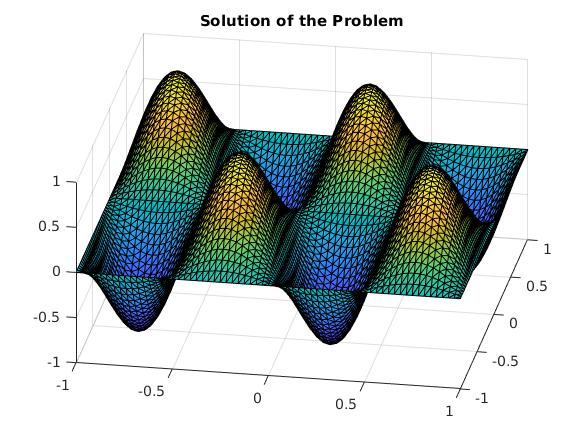
\includegraphics[width = 4in]{laplace_sol.jpg}
\caption{The computed finite element solution with $N = 8192$ triangle elements with linear basis functions.}
\label{fig:laplace_sol}
\end{figure}

\begin{figure}[H]
\centering
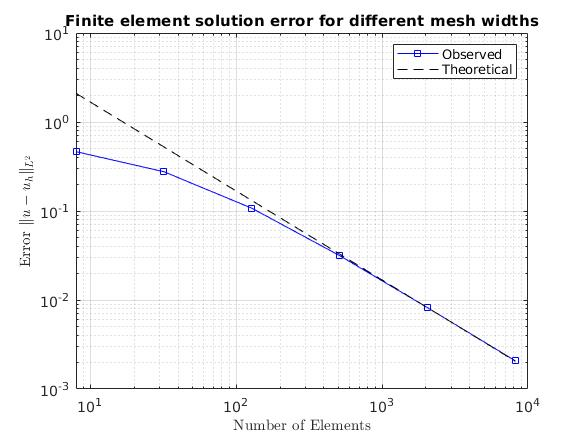
\includegraphics[width = 4in]{laplace_convergence.jpg}
\caption{The error of the finite element solution for different uniform mesh refinements (blue) compared to the theoretical convergence rate of $O(N^{-1})$ (black).}
\label{fig:laplace_convergence}
\end{figure}

%%%%%%%%%%%%%%%%%%%%%%%%%%%%%%%%%%%%%%%%%%%%%%%%%%%%%%%%%%%%%%%

\begin{figure}[h!]\centering
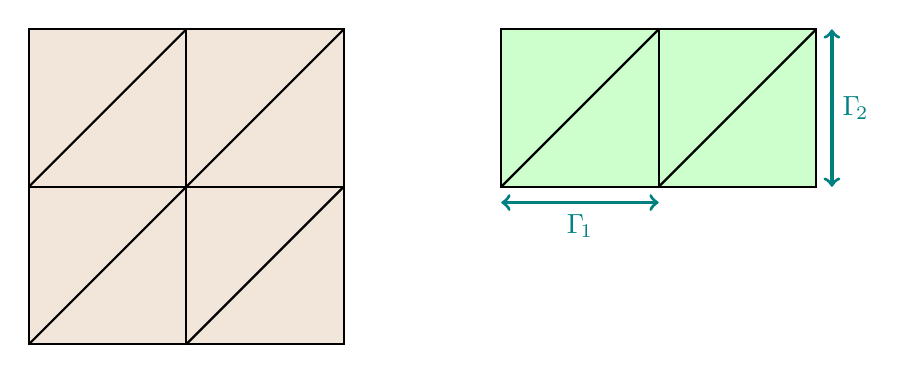
\begin{tikzpicture}
  \foreach \x in {0,2}{
    \foreach \y in {0,2}{
      \filldraw[draw=black,thick,fill=brown!20!white] (\x,\y) rectangle ++(2,2);
      \draw[draw=black,thick] (\x,\y) -- (\x+2,\y+2);
    }
  }
  \foreach \x in {0,2}{
    \foreach \y in {2}{
      \draw[draw=black,thick,fill=green!20!white] (\x+6,\y) rectangle
      ++(2,2);
      \draw[draw=black,thick] (\x+6,\y) -- (\x+8,\y+2);
    }
  }
  \node (a) at (7,1.5) {\textcolor{green!50!blue}{$\Gamma_{\!1}$}};
  \node (b) at (10.5,3) {\textcolor{green!50!blue}{$\Gamma_{\!2}$}};
  \draw[<->,very thick,green!50!blue] (6,1.8) to (8,1.8);
  \draw[<->,very thick,green!50!blue] (10.2,2) to (10.2,4);

\end{tikzpicture}
\caption{Initial discretizations for the domain
  $\Omega=[-1,1]\times[-1,1]$ (Problem 1) and domain
  $\Omega=[-1,1]\times [0,1]$ for (Problem 2).\label{fig1}}
\end{figure}


\item {\bf The Motz problem.} Let us consider the following problem
  over the domain $\Omega=[-1,1]\times [0,1]$, where we impose
  different boundary conditions (see also the right image in
  Figure~\ref{fig1}):
  \begin{alignat}{2}
    -\Delta u  &= 0 \quad &&\text{ on } \Omega,\\
    u &= 0  \quad &&\text{ on } \Gamma_{\!1}:=(-1,0)\times\{0\}, \\
    u &= 500  \quad &&\text{ on } \Gamma_{\!2}:=\{1\}\times (0,1), \\
    \frac{\partial u}{\partial n} &= 0 \quad &&\text{ on }
    \partial\Omega\setminus(\Gamma_{\!1}\cup\Gamma_{\!2}).
  \end{alignat}
  The exact solution for this problem can be written as a series
  expansion with numerically approximated coefficients. I implemented
  that solution in the file \texttt{sol\_motz.m}. Now your task is to
  update all files from the previous problem, solve the Motz problem
  on a sequence of refined meshes and plot the $L_2$ convergence
  rate. How does it compare with the theory?  To update the files:
  \begin{itemize}
    \item Number the 6 corners in the right mesh in Figure \ref{fig1},
      and update the \texttt{coordinates.dat} file. Then update the
      \texttt{elements3.dat} file to specify the 4 triangles. Be
      careful that you always order the corners anti-clockwise!
    \item Update the boundary condition files \texttt{neumann.dat} and
      \texttt{dirichlet.dat}. When you specify the edges, this must
      also be done in an anti-clockwise way as the code assumes that
      the outward pointing normal is obtained by a 90 degree
      anti-clockwise rotation!
     \item Update the Dirichlet boundary condition file
       \texttt{u\_d.m} to reflect the boundary conditions of the Motz
       problem. Also, don't forget to update \texttt{f.m}.
  \end{itemize}

%%%%%%%%%%%%%%%%%%%%%%%%%%%%%%%%%%%%%%%%%%%%%%%%%%%%%%%%%%

{\bf Solution}\\
The two figures below show the computed finite element solution for the Motz problem as well as the rate of convergence of the $L_2$ error.  We can see that the computed solution is not smooth at the point $(0,0)$ since there is a sharp change in the gradient.  Thus, $u \not \in H^2(\Omega)$ and we cannot expect the same convergence rate of $O(h^2)$ as we did before.  Instead, since $u$ is only in $H^1(\Omega)$ we can expect that $\|u - u_h\|_{L^2} = O(h)$.  This is indeed the observed rate since $h \sim N^{-1/2}$ due to being in two dimensions.

\begin{figure}[H]
\centering
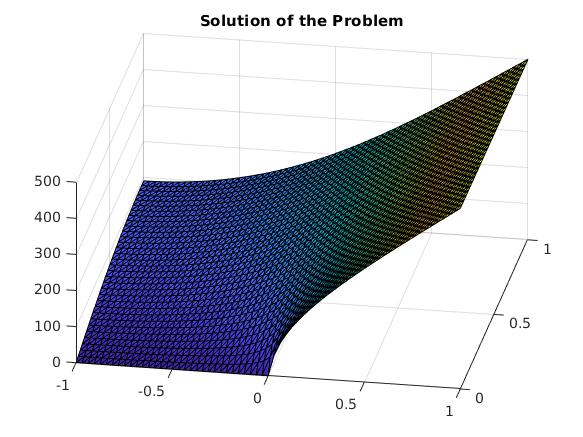
\includegraphics[width = 4in]{motz_sol.jpg}
\caption{The computed finite element solution with $N = 4096$ triangle elements with linear basis functions.}
\label{fig:motz_sol}
\end{figure}

\begin{figure}[H]
\centering
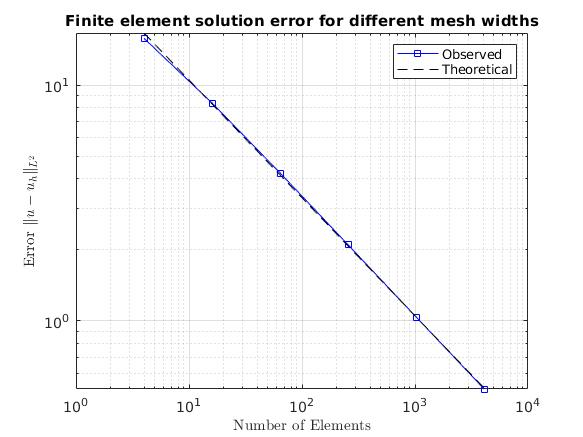
\includegraphics[width = 4in]{motz_convergence.jpg}
\caption{The error of the finite element solution for different uniform mesh refinements (blue) compared to the theoretical convergence rate of $O(N^{-1/2}) = O(h)$ (black).}
\label{fig:motz_convergence}
\end{figure}

%%%%%%%%%%%%%%%%%%%%%%%%%%%%%%%%%%%%%%%%%%%%%%%%%%%%%%%%%%



\item  {\bf A nonlinear problem.}
  As example for a nonlinear problem, let's consider the Bratu problem
  from class, where $\lambda\ge 0$:
  \begin{align*}
    u'' + \lambda e^u &= 0 \quad \text{ on } (0,1),\\
    u(0) = 0, u(1) &= 0.
  \end{align*}
The corresponding weak form is: Find $u\in V:=H_0^1(0,1)$ such that
for all $v\in V$ holds $G(u;v) = 0$, where $G(u;v)$ is the weak form
for the above problem. To solve this nonlinear problem, we follow the
linearize-then-discretize approach, i.e., we apply Newton's method for
functions and then solve each linearized problem using the finite
element method. To apply Newton's method, one can either linearize on
the strong or the weak form level. Let's do the latter, i.e., we
compute derivatives of $G$ with respect to $u$, keeping $v$ fixed.
Differentiating with respect to functions is formally similar to
standard differentiation, for instance, the directional derivative
$\delta_u G$ of $G$ in a direction $\hat u\in V$ is defined as:
\begin{equation}
 \delta_u G(u;v)(\hat u) = \lim_{\varepsilon \to 0}
 \frac{G(u+\varepsilon \hat u;v) - G(u;v)}{\varepsilon}.
\end{equation}
The Newton step, written in weak form, is then: Given $u^k\in V$, find
the Newton update $\hat u\in V$ as the solution of
\begin{equation}\label{eq:Newton-weak}
\delta_u G(u^k;v)(\hat u) = -G(u^k;v) \quad \text{ for all } v\in V.
\end{equation}
and perfom the Newton update, possibly with a damping factor $\mu\le 1$:
\begin{equation}
u^{k+1} = u^k + \mu \hat u.
\end{equation}
\begin{enumerate}
\item Compute the weak form \eqref{eq:Newton-weak} explicitly for the
  Bratu problem, and
  give the corresponding strong form.\\

%%%%%%%%%%%%%%%%%%%%%%%%%%%%%%%%%%%%%%%%%%%%%%%%%%%%%%

{\bf Solution}\\
To find the weak form of the Bratu problem we multiply by a test function $v\in V$ and integrate.
\[
\int_0^1 u''v + \lambda e^u v\ dx = \int_0^1 -u'v' + \lambda e^u v\ dx = 0 
\]
Therefore, we define
\[
G(u,v) := \int_0^1 -u'v' + \lambda e^u v\ dx
\]
for all $u,v \in V$.  Now we compute the directional derivative in a direction $\hat{u} \in V$ by
\begin{align*}
\delta_u G(u,v)(\hat{u}) &= \lim_{\varepsilon \to 0} \frac{1}{\varepsilon} \left\{ \int_0^1 -(u + \varepsilon \hat{u})'v' + \lambda e^{u + \varepsilon \hat{u}}v\ dx  -   \int_0^1 -u'v' + \lambda e^{u}v\ dx \right\}\\
&= \lim_{\varepsilon \to 0} \frac{1}{\varepsilon} \left\{  \int_0^1 -\varepsilon \hat{u}'v' + \lambda e^{u}v \left( e^{\varepsilon \hat{u}} - 1 \right)   \right\}\\
&= \int_0^1 -\hat{u}'v' + \lambda e^u v \hat{u}\ dx
\end{align*}
where the last line follows from the dominated convergence theorem and the fact that 
\[
\lim_{\varepsilon \to 0} \frac{1}{\varepsilon}\left( e^{\varepsilon \hat{u}} - 1 \right) = \hat{u}
\]
for all $x\in (0,1)$.  Thus, the weak form of the Newton update is: given $u^{k} \in V$, find $\hat{u} \in V$ such that 
\[
\int_0^1 -\hat{u}'v' + \lambda e^{u^k} v \hat{u}\ dx = - \int_0^1 -(u^k)'v' + \lambda e^{u^k} v\ dx
\]
for all $v\in V$.  This is now a linear equation for $\hat{u}$ and the right hand side does not depend on $\hat{u}$.\\

%%%%%%%%%%%%%%%%%%%%%%%%%%%%%%%%%%%%%%%%%%%%%%%%%%%%%%


\item Modify one of the implementations from one of the first
  homeworks (i.e., use either linear, quadratic or Hermite elements)
  to compute the corresponding Newton updates. For $\lambda=2$ try to
  solve Bratu's problem with the two different initializations
  $u^0\equiv 0$ and $u^0(x) = 14x(1-x)$.\footnote{It is important that
    the initialization satisfies the Dirichlet boundary conditions
    since all Newton updates have zero Dirichlet boundary
    conditions. If we search for a solution that has non-zero
    Dirichlet conditions, one can choose an initialization that
    satisfies these boundary conditions and then all updates $\hat u$
    satisfy zero Dirichlet conditions.} Try to use full Newton steps
  (i.e., $\mu=1$) and if you observe convergence problems, try
  damping, i.e., $\mu<1$. Terminate the Newton iteration when the
  update $\hat u$ is small. Report your experience and plot the
  solution(s) you find.
\end{enumerate}


\end{enumerate}




\end{document}
